\documentclass[conference]{IEEEtran}
\IEEEoverridecommandlockouts
% The preceding line is only needed to identify funding in the first footnote. If that is unneeded, please comment it out.
\usepackage{cite}
\usepackage{amsmath,amssymb,amsfonts}
\usepackage{algorithmic}
\usepackage{multirow}
\usepackage{graphicx}
\usepackage{tabularx}
\usepackage{textcomp}
\usepackage{xcolor}
\usepackage{array}
\usepackage{caption}
\usepackage[hyphens]{url}
\usepackage{hyperref}
\captionsetup[table]{skip=10pt}

\usepackage{listings}
\usepackage{color}

\definecolor{dkgreen}{rgb}{0,0.6,0}
\definecolor{gray}{rgb}{0.5,0.5,0.5}
\definecolor{mauve}{rgb}{0.58,0,0.82}

\lstset{frame=tb,
  language=Java,
  aboveskip=3mm,
  belowskip=3mm,
  showstringspaces=false,
  columns=flexible,
  basicstyle={\small\ttfamily},
  numbers=none,
  numberstyle=\tiny\color{gray},
  keywordstyle=\color{blue},
  commentstyle=\color{dkgreen},
  stringstyle=\color{mauve},
  breaklines=true,
  breakatwhitespace=true,
  tabsize=3
}

\setlength\extrarowheight{2pt}
\def\BibTeX{{\rm B\kern-.05em{\sc i\kern-.025em b}\kern-.08em
    T\kern-.1667em\lower.7ex\hbox{E}\kern-.125emX}}
\begin{document}

\title{Desempenho da Plataforma Apache Flink}

\author{\IEEEauthorblockN{João Brito, M9984}
\IEEEauthorblockA{\textit{Department of Computer Science} \\
\textit{University of Beira Interior}\\
Covilhã, Portugal \\
joao.pedro.brito\{at\}ubi.pt}
\and
\IEEEauthorblockN{André Martins, M10157}
\IEEEauthorblockA{\textit{Department of Computer Science} \\
\textit{University of Beira Interior}\\
Covilhã, Portugal \\
andremar1000\{at\}gmail.com}
}

\maketitle

\begin{abstract}
Este documento tem a função de apresentar a plataforma Apache Flink e avaliar o respetivo desempenho para dois \emph{benchmarks} diferentes. Os \emph{benchmarks} que serviram para análise desse desempenho foram o Yahoo Streaming Benchmark e o StreamBench. Será também apresentado um ponto de vista geral à arquitetura do Apache Flink, bem como um tutorial de como o instalar e configurar no sistema operativo Linux Ubuntu.
\end{abstract}

\section{Introdução}
\label{intro}

O Apache Flink é uma plataforma processamento de fluxo \emph{open-source} desenvolvido pela Apache Software Foundation. É uma plataforma escrita em Java e Scala e executa, de uma maneira arbitrária, programas de forma paralela e canalizada. É uma ferramenta muito utilizada na área de \emph{Big Data} e tem vários pontos que o tornam ideal na área do processamento de grandes quantidades de dados:

\begin{itemize}
    \item É uma \emph{"true stream processing framework"}, ou seja, não corta o fluxo em micro-\emph{batches};
    \item O núcleo do Flink tem a capacidade de processamento distribuído, tolerância a falhas, entre outros;
    \item Processa eventos a uma velocidade elevada, com baixa latência;
    \item É uma plataforma de processamento de dados de larga escala com capacidade de processar um grande volume de dados.
\end{itemize}

É também uma plataforma que responde a vários requisitos de uma maneira bastante eficaz e eficiente, nomeadamente:

\begin{itemize}
    \item \emph{Batch Processing};
    \item \emph{Interactive Processing};
    \item \emph{Real-time stream processing};
    \item \emph{Graph processing}.
\end{itemize}

É cada vez mais utilizado como uma alternativa ao \emph{MapReduce}, usado no Hadoop, e consegue processar dados 100 vezes mais rápido que o \emph{MapReduce}. Pode utilizar o HDFS do Hadoop para ler, escrever, guardar e processar dados e não tem um sistema de armazenamento dos mesmos.

Devido a todas estas funcionalidades descritas, vários desenvolvedores desenvolveram os mais diversos \emph{benchmarks} de modo a medir a eficiência que o Apache Flink apresenta durante o processamento de dados. O Yahoo Streaming Benchmark e o StreamBench são dois \emph{benchmarks} de referência que permitem então fazer essa análise ao Apache Flink e foram utilizadas para o desenvolvimento deste estudo. 

\section{Arquitetura do Apache
Flink}
\label{arquitetura}

Todos os tipos de dados são produzidos através de um fluxo de eventos, como por exemplo, transações de um cartão de crédito ou medidas registadas por sensores. Todos estes dados são gerados como um fluxo. Como tal, podem ser processados de duas maneiras distintas:

\begin{itemize}
    \item Fluxo ilimitado;
    \item Fluxo limitado.
\end{itemize}

O fluxo ilimitado, tal como o nome sugere, tem um início mas não tem um fim definido. É um fluxo que nunca termina e está sempre a providenciar dados enquanto ele é gerado. Os eventos gerados por este fluxo devem ser sempre manuseados depois de terem sido processados pelo sistema. Visto que é ilimitado, é impossível esperar pela chegada de todos os dados pois estes nunca vão estar completos. Como tal, o seu processamento requer que os eventos sejam processados com um determinado critério de ordenação (e.g. instante em que se registou cada evento).

Por outro lado, o fluxo limitado carateriza-se por estar bem delimitado, tendo início e fim. Todos os dados presentes neste tipo de fluxo são processados antes de existir qualquer tipo de computação relacionada com eles. O processamento deste tipo de dados é também conhecido como \emph{batch processing}.

A figura seguinte apresenta um gráfico que dá a entender o formato de ambos os tipos de fluxos, sendo possível ver a grande diferença entre eles e como é que estes se encontram ao longo de um fluxo de dados:

\begin{figure}[!htbp]
\centering
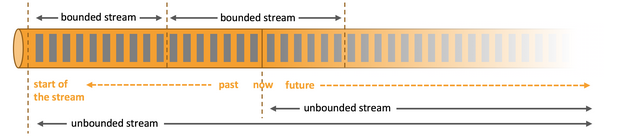
\includegraphics[scale= 0.55]{fluxos.png}
\caption{Fluxos ilimitados e limitados.}
\label{fluxos}
\end{figure}

Os dois conceitos anteriores são importantes pois o Apache Flink destaca-se no processamento de bases de dados limitadas e ilimitadas, devido ao preciso controlo do tempo e estado. Graças a esse controlo, é possível à plataforma correr qualquer tipo de fluxo ilimitado sem grandes complicações. Já os fluxos limitados, são processados internamente através de algoritmos e estruturas de dados desenhados para bases de dados com um tamanho fixo, aumentando assim a performance da plataforma.

Visto que o Apache Flink é um sistema distribuído e requer recursos computacionais de modo a que possa executar aplicações, está integrado com vários \emph{softwares} de gestão de recursos em \emph{cluster}, como é o caso do Apache Mesos e dos Kubernetes. No entanto, também pode ser executado de uma maneira independente.

Quando é lançada uma aplicação, a plataforma identifica automaticamente os recursos necessários baseado nas configurações da aplicação, sendo que esse pedido é feito então ao gestor de recursos. Toda esta comunicação é feita através de chamadas REST, um estilo de arquitectura de software que define um conjunto de restrições a serem usadas para a criação de serviços Web, o que facilita a integração nos mais diversos ambientes.

Permite também correr milhares de tarefas em paralelo e de maneira distribuída por vários \emph{clusters}, o que permite às aplicações usarem uma quantidade ilimitada de recursos, como tempo de CPU, memória principal ou até mesmo rede.

Por último, as aplicações são otimizadas para acesso local. O estado da tarefa é mantido na memória principal da máquina e, sempre que excede o limite, acede às estruturas presentes no disco. Devido a todos os acessos serem locais, a latência do processamento é extremamente baixa. O Apache Flink garante então a consistência dos estados em caso de falha, através de mecanismos de \emph{backup} que guardam o estado local da aplicação na memória da máquina. Todo este processo está representado na seguinte figura.

\begin{figure}[!htbp]
\centering
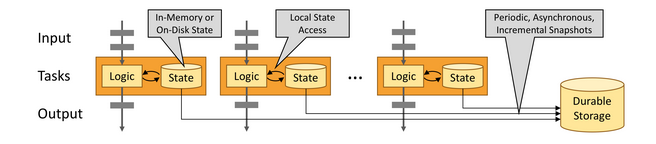
\includegraphics[scale= 0.5]{memory.png}
\caption{Metodologia de acesso local das aplicações.}
\label{memory}
\end{figure}

\section{Instalação e Configuração do Flink}
\label{instalacao}

A instalação da plataforma Apache Flink foi feita para o sistema operativo Linux Ubuntu, versão 20.04. Esta plataforma necessita de várias funcionalidades/dependências extra para ser executada devidamente. Destas, destaca-se, em primeiro lugar, o interpretador Python, que pode ser instalado usando o seguinte comando:

\begin{lstlisting}[language=bash]
  $ sudo apt-get install python-software-properties 
\end{lstlisting}

A segunda funcionalidade é o Java, um dos componentes principais para que o Apache Flink seja executado sem qualquer erro. Primeiramente, é preciso instalar o JRE (\emph{Java Runtime Environment}) usando o comando:

\begin{lstlisting}[language=bash]
  $ sudo apt install default-jre
\end{lstlisting}

De seguida, é preciso também instalar o JDK (\emph{Java Development Kit}), através do comando:

\begin{lstlisting}[language=bash]
  $ sudo apt install default-jdk
\end{lstlisting}

Após os passos anteriormente descritos, passamos então à instalação do Apache Flink.

O primeiro passo é fazer o \emph{download} do ficheiro ".tar" do site oficial da plataforma.

De seguida, é necessário fazer a descompressão desse ficheiro, que pode ser feita através do comando:

\begin{lstlisting}[language=bash]
  $ tar xzf flink-<version>-bin-hadoop26-scala_2.11.tgz
\end{lstlisting}

onde $<version>$ é o número da versão da plataforma que foi descarregada.

Após a descompressão, é originada uma pasta na mesma directoria com o nome "flink-X", onde $X$ é o número da versão do Apache Flink.

Por último, através do terminal, navega-se até à pasta "bin" dentro da pasta de instalação da plataforma e executa-se o ficheiro "start-clusters.sh", através do comando:

\begin{lstlisting}[language=bash]
  $ ./start-local.sh
\end{lstlisting}

Após todos estes passos, o Apache Flink está pronto a ser utilizado e considera-se como configurado. Para verificar que está operacional, pode-se aceder à Web UI oferecido pelo Apache Flink, que terá um aspeto semelhante ao da seguinte figura:

\begin{figure}[!htbp]
\centering
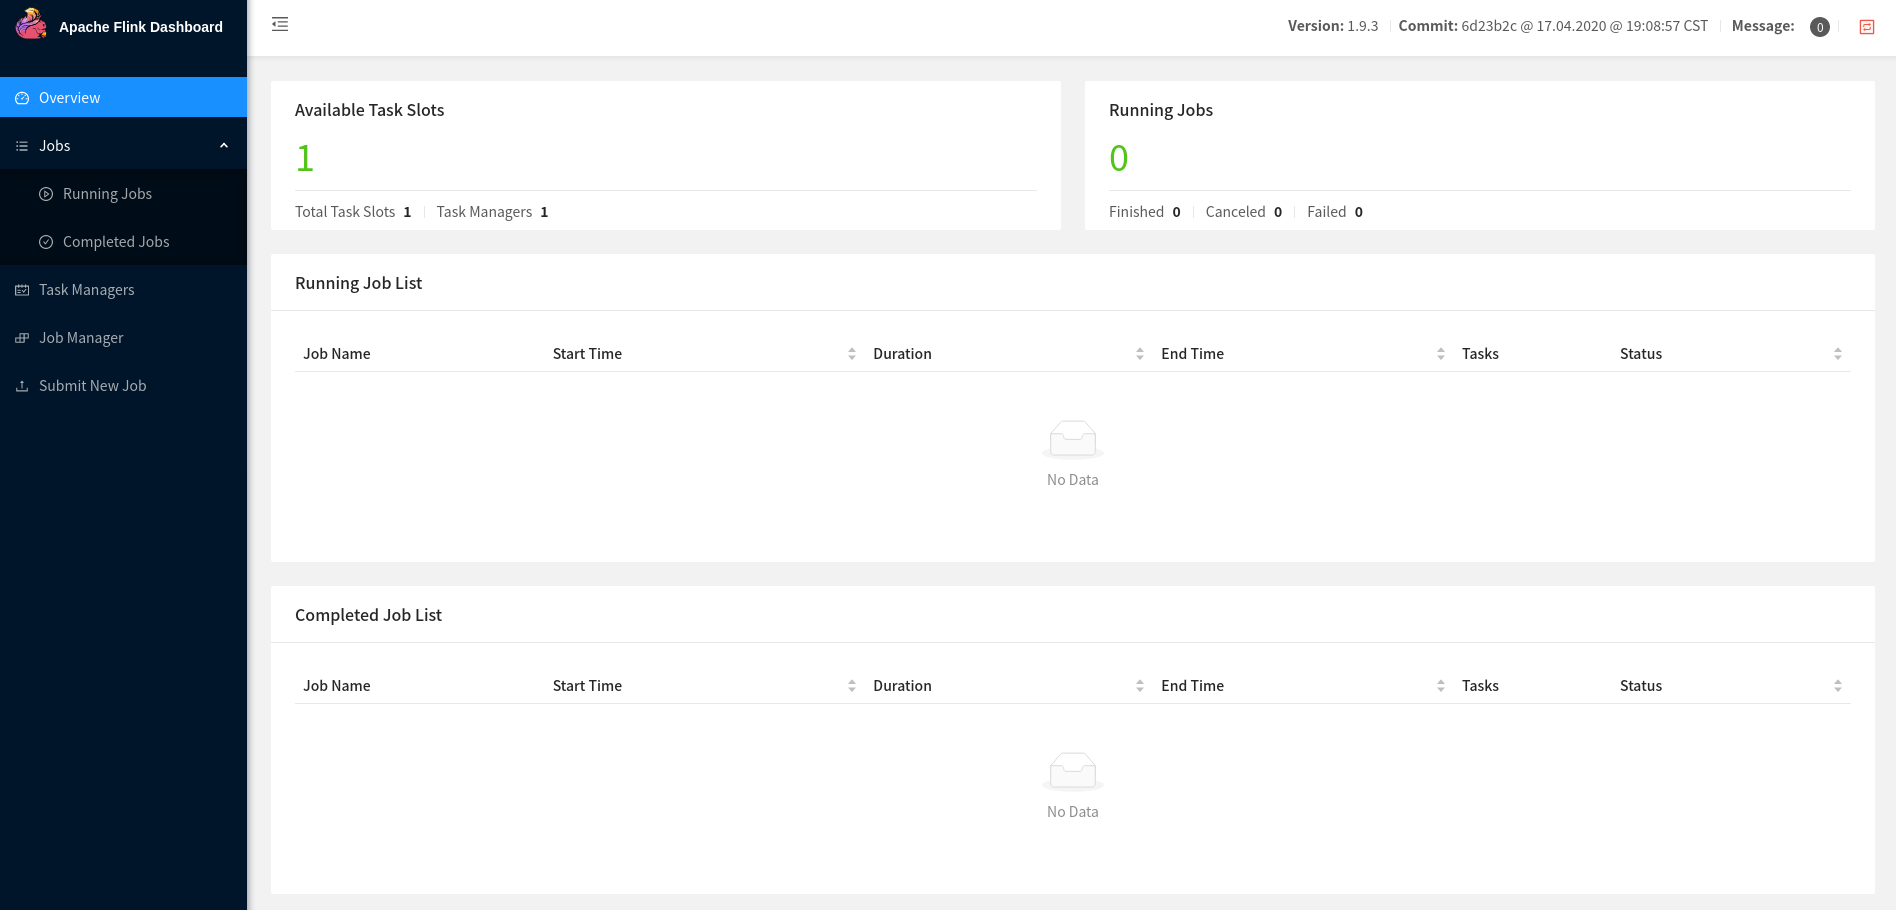
\includegraphics[scale=0.130]{webui.png}
\caption{Web UI do Apache Flink.}
\label{WebUi}
\end{figure}

Também é possivel fazer essa verificação através do comando "jps", cuja saída da sua execução será semelhante à seguinte:

\begin{lstlisting}[language=bash]
  3814 StandaloneSessionClusterEntrypoint
  4343 Jps
  4249 TaskManagerRunner
\end{lstlisting}

\section{Benchmarks Usados para Avaliação
do Desempenho}
\label{benchmarks}

A presente secção terá como foco a descrição discussão de detalhes de implementação dos dois \emph{benchmarks} utilizados para avaliação de desempenho do Apache Flink.

\subsection{Yahoo Streaming Benchmark}
\label{yahoo}

O Yahoo Streaming Benchmark foi um programa previamente desenvolvido para correr juntamente com o Apache Storm. No entanto, com o decorrer dos anos, foi necessário começar a desenvolver um benchmark que corre-se juntamente com outras tecnologias, que tivessem maior rendimento e performance que o Apache Storm. Desta maneira, podia começar-se a dar recomendações aos clientes de qual a melhor ferramenta a ser usada em diversas situações. 

Assim, foi desenvolvido este \emph{benchmark}, que tem algumas funcionalidades úteis e que devolvem alguns resultados que podem ser analisados. No entanto, e como os próprios desenvolvedores afirmam, o programa desenvolvido tem problemas no que toca a abordar diversos aspetos de áreas fundamentais, pois não tem uma aplicação real, sendo apenas um desenvolvimento básico para alguns testes. Como tal, esta ferramenta apenas aborda um caso específico.

Começando então com a instalação e configuração do \emph{benchmark}, é necessária a instalação de dois pré-requisitos: o software "Maven" e o software "Leiningen". Os seguintes comandos produzem esse efeito:

\begin{lstlisting}[language=bash]
  $ sudo apt-get install maven
  
  $ sudo apt-get install leiningen
\end{lstlisting}

Após esta instalação, procede-se à execução do ficheiro "stream-bench.sh". A sua execução apresenta um menu de argumentos que podem ser utilizados aquando da sua execução. Como tal, o primeiro passo é fazer o \emph{setup}, através do comando:

\begin{lstlisting}[language=bash]
  $ ./stream-bench.sh SETUP
\end{lstlisting}

Durante o setup poderão encontrar-se vários problemas. O primeiro problema ocorrer se o programa estiver a ser executado num JRE. Tal inviabiliza o \emph{setup}, visto que este precisa de ser executado no JDK. Como tal, é preciso fazer essa mudança, sendo que uma possibilidade é desinstalar o Java e reinstalar apenas o JDK. É aconselhado o uso da versão 8. 

O segundo problema encontrado foi a lentidão das transferências dos repositórios relativos ao software "APEX", uma vez que estes já não se encontravam disponíveis para \emph{download} no \emph{website} recomendado. Como tal, e visto que o "APEX" não era necessário, eliminou-se do código fonte tudo o que era relacionado com esse \emph{software}, de maneira a aumentar a velocidade da compilação e execução do \emph{setup}. 

De resto, todas as transferências necessárias foram realizadas, bem como os demais passos, culminando no correto \emph{setup} deste \emph{benchmark} (finalizado com uma mensagem de sucesso).

Um facto a ter em conta é que este \emph{benchmark} traz a sua própria instalação do Apache Flink, usando assim a versão 1.6.0 do \emph{software}.

O próximo passo corresponde à inicialização do Apache Flink, com recurso ao comando:

\begin{lstlisting}[language=bash]
  $ ./stream-bench.sh START_FLINK
\end{lstlisting}

Deste modo, o servidor é inicializado, possibilitando a execução do programa com o Apache Flink.

Por último, é então executado o teste:

\begin{lstlisting}[language=bash]
  $ ./stream-bench.sh FLINK_TEST
\end{lstlisting}

Durante esta execução, são inicializados os servidores "Zookeeper", "Redis" e "Kafka", de modo a que a execução do teste seja bem sucedida. Um possível problema é a Virtual Machine do Java não ser bem inicializada, o que pode indicar que a versão do Java que está a ser utilizada não é a correta. Se este problema não ocorrer, vão ser então apresentados os resultados respetivos da execução do teste.

De notar que durante a execução, se acedermos ao \emph{dashboard} do Apache Flink é possível acompanhar toda a execução do projeto em tempo real.

\subsection{StreamBench}
\label{stream}

O StreamBench é um projeto que mede a performance de plataformas de \emph{streaming} populares.

Durante a execução do projeto, é comparada a performance da plataforma "SABER", uma plataforma eficiente de processamento de fluxo de dados, usando dois sistemas de processamentos de dados: o Apache Spark e o Apache Flink. No entanto, para a análise efetuada apenas se vão ter em conta os resultados dados pelo Apache Flink. Também vai ser avaliada outra plataforma, a "StreamBox", que é uma plataforma que faz processamento de dados sem ordem num único servidor.

Para ser possível correr este benchmark, foi necessária a instalação do software "Maven", através do comando:

\begin{lstlisting}[language=bash]
  $ sudo apt-get install maven
\end{lstlisting}

De seguida, sendo que o Apache Flink já está a ser executado, foi preciso entrar na pasta "Flink", presente na pasta principal do \emph{benchmark} e executar o ficheiro "run\textunderscore flink.sh", através dos comandos:

\begin{lstlisting}[language=bash]
  $ cd /StreamBench/flink
  
  $ ./run_flink.sh
\end{lstlisting}

Durante a execução deparou-se com um erro no qual o programa não encontrava classes necessárias à sua execução. Constatou-se que existia incompatibilidade do programa com a versão 11 do Java e, como tal, fez-se um \emph{downgrade} para a versão 8, de modo a que fosse possível fazer a execução do programa.

Por último foram efetuadas as transferências de diversos módulos e repositórios necessários, sendo que após todo este processo começaram a ser dadas informações sobre a capacidade de processamento de dados e de latência durante o processamento efectuado pelo programa. Os resultados obtidos serão apresentados na seguinte secção.

\section{Experiências e Resultados}
\label{resultados}

\subsection{Yahoo Streaming Benchmark}
\label{yahoo}

Para o \emph{benchmark} da Yahoo, só foi possível obter valores de latência, uma vez que, na sua versão atual e testada, não está implementada qualquer métrica de \emph{throughput} (capacidade de processamento). 

A figura seguinte apresenta um excerto do \emph{output} produzido por este \emph{benchmark}:

\begin{figure}[!htbp]
\centering
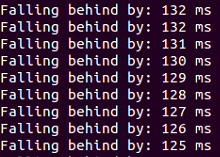
\includegraphics[scale=0.930]{Relatorio/imgs/bench2lat.png}
\caption{Valores de latência para o Yahoo Streaming Benchmark.}
\label{yahoo_res}
\end{figure}

Como é constatado na figura \ref{yahoo_res}, este \emph{benchmark} apresenta valores de latência consideráveis, o que pode condicionar a eficiência do mesmo em aplicações reais. De notar, que a imagem referida apresenta valores para um dos testes efetuados. Em outras instâncias de teste, os valores de latência chegaram a um mínimo de 101ms, sendo ainda elevado para o pretendido.

\subsection{StreamBench}
\label{stream}

Por sua vez, este \emph{benchmark} apresenta valores de latência e \emph{throughput}, como se pode observar na seguinte figura:

\begin{figure}[!htbp]
\centering
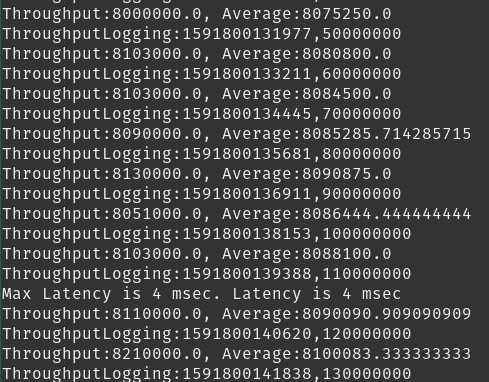
\includegraphics[scale=0.430]{Relatorio/imgs/bench1res.png}
\caption{Valores de latência e \emph{throughput} para o StreamBench.}
\label{stream_res}
\end{figure}

De acordo com os resultados obtidos, podemos constatar que, para diversas aplicações, um servidor de vários núcleos aplicado a um \emph{cluster} tem uma melhor capacidade de processamento de fluxo de dados do que um servidor que usa vários \emph{clusters}. Tal situação abre uma janela de oportunidade para que se reduzam custos operacionais ao substituir sistemas com vários nós de processamento.

\subsection{Avaliação Comparativa}
\label{yahoo}

Com base nos resultados apresentados nas secções anteriores, podem-se derivar as seguintes conclusões:

\begin{itemize}
    \item O \emph{benchmark} StreamBench parece superiorizar-se em relação ao Yahoo Streaming Benchmark, reportando valores de latência bastante inferiores (o que é, naturalmente, uma propriedade desejável).
    \item O \emph{benchmark} da Yahoo apresenta algumas lacunas em termos de implementação, concretizando-se na falta de mais métricas de desempenho (\emph{throughput}) e/ou de outras funcionalidades fundamentais.
    \item Seguindo o ponto anterior, o StreamBench conta com mais métricas de avaliação, o que é benéfico e útil (particularmente para um estudo comparativo como o que se descreve no presente documento).
\end{itemize}

\section{Conclusão}
\label{conclusao}

O documento descrito procurou descrever, num primeiro momento, a arquitetura do Apache Flink e avaliar a sua performance com dois \emph{benchmarks} distintos. No decurso da execução destes, foram encontrados alguns problemas, normalmente associados ao Java e às suas versões. Tal detalhe é claramente um fator a considerar em projetos de natureza semelhante.

A nível mais prático e com base nos testes realizados, pode-se afirmar que o StreamBench é superior ao equivalente da Yahoo, não só pelas funcionalidades a mais como pelos valores de latência inferiores. Deve, portanto, ser priorizado em aplicações reais.

Por fim, e tendo em conta que o projeto aqui descrito tem um caráter introdutório, as conclusões reportadas poderão ser complementadas e reforçadas num trabalho futuro, com a realização de mais testes e avaliação de outros \emph{benchmarks}.

%referir que se teve bastantes problemas na execução dos benchmarks, muitos deles relativos com o java.
%concluir que o streambench e melhor para muitas aplicaçoes reais
% algum trabalho futuro tipo explorar mais a fundo cada um dos benchmarks para obter outros resultados, fazer outros testes e usar outros benchmarks.

\begin{thebibliography}{00}

\bibitem{b1} Download Apache Flink [Online] \url{https://flink.apache.org/downloads.html}
\bibitem{b2} Download StreamBench [Online] \url{https://github.com/lsds/StreamBench}
\bibitem{b3} Download Yahoo Streaming Benchmark [Online] \url{https://github.com/yahoo/streaming-benchmarks}
\bibitem{b4} Instalar Flink no Ubuntu [Online] \url{https://data-flair.training/blogs/apache-flink-installation-on-ubuntu/}
\bibitem{b5} Arquitetura Apache Flink [Online] \url{https://flink.apache.org/flink-architecture.html}

\end{thebibliography}

\end{document}
